\documentclass{article}

\usepackage[letterpaper]{geometry}
\usepackage{graphicx}

\graphicspath{{./img/}}

\title{2411 HW 9}
\author{Duncan Wilkie}
\date{12 November 2021}

\begin{document}

\maketitle

\section{}
The interpolation used in figure 1.12 is regression from an expected curve, where they determined the parameters necessary for a function of a given type to go through the data points reasonably well. The dashed curve is again regression. It is done via the same mechanism described above, and finds the mass of the $Z$ boson since that is expected to be one of the parameters of the function that is being fitted. The result is a quite good fit, with a relative uncertainty of two thousandths of a percent in the quantity of interest and errors of similar magnitude elsewhere. The mass found is $91.1875\pm { 0.0021}{GeV}$.

\section{}
The program appears in the script files.
The graph of the distribution appears below.
\[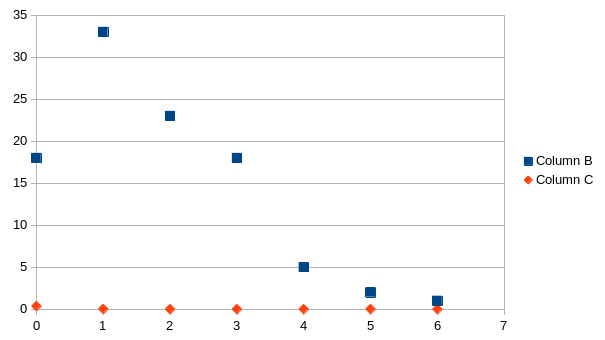
\includegraphics[scale=0.5]{plot.png}\]
\section{}
The estimate for the population mean is simply the mean of the sample, $\mu ={0.636}{s}$. The estimate of the population variance is $\sigma^2 = \frac{n-1}{n}s^2=\frac{99}{100}(0.014)^2\Rightarrow \sigma={0.0139}{s}$

\section{}
The program written appears in the script files section. The period of both generators is 9, since the congruence is modulo 9. The range in the first case is integers from 0 to 8, and in the second case is those integer multiples of $1/8$.

\section{Script Files}
\begin{verbatim}
#include <iostream>
#include <fstream>

using namespace std;

int main() {
  ofstream out;
  out.open("output1.txt");
  int x = 3;

  for (int i = 0; i < 12; i++) {
    out << x << endl;
    x = (4 * x + 1) % 9;
  }

  return 0;

}

\end{verbatim}

\begin{verbatim}
#include <iostream>
#include <fstream>

using namespace std;

int main() {
  ofstream out;
  out.open("output2.txt");
  int x = 3;

  for (int i = 0; i < 12; i++) {
    out << (float)x / 8 << endl;
    x = (4 * x + 1) % 9;
  }

  return 0;

}

\end{verbatim}

\begin{verbatim}
#include <iostream>
#include <cmath>

using namespace std;

int main() {

  int y[7] = {18, 33, 23, 18, 5, 2, 1};

  int ctotal = 0, itotal = 0;
  for (int i = 0; i < 7; i++) {
    ctotal += i*y[i];
    itotal += y[i];
  }

  double mean = ctotal / itotal;

  double stdv = 0;
  for (int i = 0; i < 7; i++) {
    stdv = sqrt(pow(stdv, 2) + pow(y[i]-mean, 2));
  }

  stdv /= sqrt(itotal);

  cout << "The estimated population mean is " << mean << endl;
  cout << "The standard deviation is " << stdv << endl;

  double P = exp(-mean);
  for (int i = 0; i < 7; i++) {
    cout << P << endl;
    P *= mean / y[i];
  }
  return 0;

}

\end{verbatim}
\end{document}
%%% Local Variables:
%%% mode: latex
%%% TeX-master: "report"
%%% End:
